\documentclass[conference]{IEEEtran}
\IEEEoverridecommandlockouts

\usepackage{cite}
\usepackage{amsmath,amssymb}
\usepackage{graphicx}
\usepackage{booktabs}
\usepackage{algorithm}
\usepackage{algpseudocode}
\usepackage{tikz}
\usetikzlibrary{arrows.meta,fit}
\usepackage{url}

\begin{document}

\title{CloudMARL: Decentralized Load Balancing Across Heterogeneous Cloud VMs with Independent Multi-Agent Q-Learning}

\author{\IEEEauthorblockN{Anuran Baruah}
\IEEEauthorblockA{\textit{[Department]} \\
\textit{[Institution]}\\
[City], [Country] \\
baruahanuran@gmail.com}
}

\maketitle

\begin{abstract}
Geo-distributed cloud services route requests through several regional load balancers that share one pool of virtual machines (VMs). Static policies such as round-robin ignore VM capacity, and centralized optimizers need global, up-to-date state. This paper presents CloudMARL, a system in which every regional load balancer is an independent tabular Q-learning agent. Each agent observes only a coarse load level of every VM, chooses the VM for each job, and is rewarded with the negative of the job's end-to-end latency. The agents share no Q-tables and exchange no messages. CloudMARL is implemented as containerized microservices (FastAPI workers and balancers, a PostgreSQL-backed cloud API, and a Grafana dashboard) and is publicly available. In an experiment with four regions, five heterogeneous VMs and 68\% offered load, the learning agents reduced mean job latency by 58.4\% and 95th-percentile latency by 42.1\% compared with the best static baseline, and reduced the fraction of rejected jobs from 11.25--12.69\% to 1.53\%. Starting from a random policy, the agents' exploration rate reached its floor within 43~s. We also discuss the limits of the study, including emulated network delay, a single-host testbed, and baselines that are unaware of capacity.
\end{abstract}

\begin{IEEEkeywords}
cloud computing, load balancing, multi-agent reinforcement learning, Q-learning, microservices
\end{IEEEkeywords}

\section{Introduction}
Cloud applications serve users from many regions. Requests usually enter through a regional load balancer, which forwards each one to a backend VM. In practice the backend pool is heterogeneous: VMs of different instance sizes are provisioned at different times, and the network distance from each region to each VM differs. A good routing policy must therefore weigh two quantities that pull in different directions, the queueing delay of a VM (which depends on its capacity and on what every other balancer sends to it) and the network delay to reach it.

Simple policies such as round-robin and random assignment are popular because they need no state, but they are blind to capacity: a VM with two worker slots receives the same share of traffic as a VM with seven. Load-aware policies such as join-the-shortest-queue or the power of two choices~\cite{mitzenmacher2001} work well when one dispatcher has fresh queue information, but several independent dispatchers that act on the same snapshot can all choose the same lightly loaded server and overload it, a herd effect caused by stale load information~\cite{mitzenmacher2000old}.

Reinforcement learning (RL) offers a different route: a dispatcher can learn the consequences of its routing choices directly from observed latency, without an explicit model of capacities or delays~\cite{sutton2018,mao2016deeprm}. With several regional dispatchers this becomes a multi-agent reinforcement learning (MARL) problem~\cite{busoniu2008}. Each agent's best action depends on the actions of the others, so from any single agent's point of view the environment is non-stationary~\cite{hernandezleal2017}.

This paper studies the simplest form of MARL for this setting, \emph{independent learners}~\cite{tan1993,claus1998}, implemented as a working cloud system rather than a pure simulation. The contributions are:
\begin{enumerate}
\item A formulation of regional request routing as an independent multi-agent Q-learning problem with a compact, capacity-normalized state (Section~\ref{sec:model}).
\item CloudMARL, a publicly available implementation of the formulation as containerized microservices with persistent telemetry and a live monitoring dashboard (Section~\ref{sec:system}).
\item An experimental comparison with round-robin and random routing on identical workloads, together with an analysis of the routing behaviour the agents learned (Sections~\ref{sec:setup}--\ref{sec:results}).
\end{enumerate}

\section{Background and Related Work}
\subsection{Load balancing in the cloud}
Production load balancers combine fast, stateless spreading with health checking, for example consistent hashing in Google's Maglev~\cite{eisenbud2016maglev}. For queueing-aware dispatch, the power of two choices~\cite{mitzenmacher2001} sharply reduces maximum load by sampling two servers and choosing the shorter queue. Join-Idle-Queue~\cite{lu2011jiq} addresses the case of many parallel dispatchers by having idle servers announce themselves, which avoids the herd effect without per-request probing. These methods assume homogeneous servers or require explicit weights for heterogeneous ones. CloudMARL learns such weights implicitly from latency feedback.

\subsection{Reinforcement learning for resource management}
Q-learning~\cite{watkins1992} learns an action-value function $Q(s,a)$ from sampled transitions and converges to the optimal policy of a stationary Markov decision process under standard conditions. Deep RL extended the approach to large state spaces~\cite{mnih2015dqn}, and DeepRM~\cite{mao2016deeprm} showed that a policy-gradient agent can learn cluster job scheduling that competes with hand-tuned heuristics. These works use a single, centralized agent.

\subsection{Multi-agent reinforcement learning}
When several agents learn at the same time, each agent's transition and reward functions depend on the others' changing policies~\cite{busoniu2008,hernandezleal2017}. Tan~\cite{tan1993} compared independent and cooperative Q-learners, and Claus and Boutilier~\cite{claus1998} analysed the dynamics of independent learners in cooperative games. Later methods such as MADDPG~\cite{lowe2017maddpg} use centralized training with decentralized execution to counter non-stationarity. CloudMARL deliberately stays with fully independent, tabular learners. They are cheap, easy to inspect, and need no coordination channel, which makes them a useful baseline for more advanced MARL methods in this domain.

\section{System Model and MARL Formulation}\label{sec:model}
\subsection{Environment}
Let $\mathcal{R}$ be the set of regions, each served by one load balancer, and $\mathcal{W}$ the set of VMs ($|\mathcal{R}|=4$, $|\mathcal{W}|=5$ in our experiments). Jobs arrive at region $r$ as a Poisson process with rate $\lambda_r$. VM $w$ has $c_w$ parallel slots; each job's service time is exponentially distributed with mean $1/\mu = 200$~ms, so the VM can complete at most $c_w\mu$ jobs per second. Jobs that find all slots busy wait in a FIFO queue. A VM rejects a job when it already holds $c_w + 40$ jobs (admission control) or when it is down. Routing a job from region $r$ to VM $w$ adds a network delay $d_{r,w}$. The end-to-end latency of a job is therefore
\begin{equation}
L = d_{r,w} + T^{\text{queue}}_w + T^{\text{service}}.
\end{equation}
Table~\ref{tab:env} lists the capacities and delays used in this study. The pool's total capacity is $\sum_w c_w\mu = 100$ jobs/s.

\begin{table}[t]
\caption{VM capacities and added network delay $d_{r,w}$ (ms)}
\label{tab:env}
\centering
\begin{tabular}{@{}lccccc@{}}
\toprule
 & vm-xl & vm-l & vm-m & vm-s1 & vm-s2 \\
Slots $c_w$ & 7 & 5 & 4 & 2 & 2 \\
Max rate (jobs/s) & 35 & 25 & 20 & 10 & 10 \\
\midrule
Mumbai    & 30  & 50  & 120 & \textbf{20} & 150 \\
Singapore & 40  & \textbf{30}  & 100 & 80  & 140 \\
Frankfurt & 100 & 120 & \textbf{30}  & 110 & 50  \\
Virginia  & 140 & 150 & 60  & 160 & \textbf{20} \\
\bottomrule
\end{tabular}
\\[2pt]{\footnotesize Bold: nearest VM for each region.}
\end{table}

\subsection{Agents, states, actions and rewards}
Each region's load balancer is an independent agent $i \in \mathcal{R}$ with its own Q-table.

\textbf{State.} Agent $i$ periodically polls every VM for its number of jobs in the system $n_w$ and its health. It maps each VM to one of three load levels,
\begin{equation}
b_w = \begin{cases}
0 & n_w / c_w < 0.75 \quad \text{(idle)}\\
1 & 0.75 \le n_w / c_w < 1.5 \quad \text{(busy)}\\
2 & n_w / c_w \ge 1.5 \text{ or VM down} \quad \text{(saturated)}
\end{cases}
\end{equation}
and uses $s = (b_1,\dots,b_{|\mathcal{W}|})$ as its state, giving $3^5 = 243$ states. Normalizing by $c_w$ makes the state comparable across VM sizes.

\textbf{Action.} The action $a \in \mathcal{W}$ is the VM that receives the current job.

\textbf{Reward.} When the job completes, the agent receives $r = -L$ (in seconds), or $r = -5$ if the job was rejected or timed out. The reward is local: each agent sees only the latency of its own jobs.

\textbf{Learning rule.} After each job the agent applies the Q-learning update~\cite{watkins1992}
\begin{equation}
Q_i(s,a) \leftarrow Q_i(s,a) + \alpha\big[r + \gamma \max_{a'} Q_i(s',a') - Q_i(s,a)\big],
\end{equation}
where $s'$ is the agent's observed state when the job completes. We use $\alpha = 0.1$ and $\gamma = 0.3$; the low discount reflects that one routing decision has little effect on the distant future. Q-values start at $0$, which is optimistic because all rewards are negative, so untried actions are still tried under a greedy policy.

\textbf{Exploration.} Actions are chosen $\varepsilon$-greedily. $\varepsilon$ starts at $1$ and is multiplied by $0.995$ after every decision down to $0.02$, which takes about $780$ decisions. When a VM's health status changes, the agent sets $\varepsilon \leftarrow \max(\varepsilon, 0.3)$ so that it re-explores after failures and recoveries.

Algorithm~\ref{alg:agent} summarizes one agent.

\begin{algorithm}[t]
\caption{Regional load balancer agent $i$}
\label{alg:agent}
\begin{algorithmic}[1]
\State $Q_i(s,a) \gets 0$ for all $s,a$; \ $\varepsilon \gets 1$
\State In background: every 100 ms poll all VMs, update $(n_w, \text{up}_w)$; if any $\text{up}_w$ changed, $\varepsilon \gets \max(\varepsilon, 0.3)$
\For{each arriving job}
  \State $s \gets \text{encode}(n, \text{up})$
  \State $a \gets$ random VM with probability $\varepsilon$, else $\arg\max_a Q_i(s,a)$
  \State $\varepsilon \gets \max(0.02,\ 0.995\,\varepsilon)$; \ $n_a \gets n_a + 1$
  \State send job to VM $a$ after delay $d_{i,a}$; measure latency $L$
  \State $r \gets -L$ if served, else $-5$; \ $s' \gets \text{encode}(n, \text{up})$
  \State $Q_i(s,a) \gets Q_i(s,a) + \alpha[r + \gamma\max_{a'}Q_i(s',a') - Q_i(s,a)]$
\EndFor
\end{algorithmic}
\end{algorithm}

\section{CloudMARL Design and Implementation}\label{sec:system}
Fig.~\ref{fig:arch} shows the architecture. All services are written in Python and packaged in one container image; Docker Compose starts the full stack of 12 services.

\begin{figure}[t]
\centering
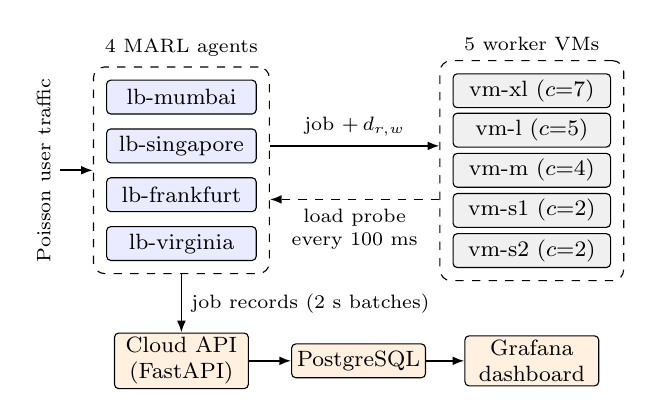
\begin{tikzpicture}[font=\footnotesize,
  box/.style={draw, rounded corners=1.5pt, minimum height=4.3mm, inner sep=1.5pt, align=center},
  agent/.style={box, fill=blue!8, minimum width=19mm},
  vm/.style={box, fill=gray!12, minimum width=20mm},
  svc/.style={box, fill=orange!12, minimum width=17mm},
  arr/.style={-{Latex[length=1.5mm]}, semithick}]
\node[agent] (m) at (0,0)     {lb-mumbai};
\node[agent] (s) at (0,-0.62) {lb-singapore};
\node[agent] (f) at (0,-1.24) {lb-frankfurt};
\node[agent] (v) at (0,-1.86) {lb-virginia};
\node[draw, dashed, rounded corners, inner sep=1.6mm, fit=(m)(v),
      label={[font=\scriptsize]above:4 MARL agents}] (A) {};
\node[vm] (w1) at (4.45,0.08)  {vm-xl ($c{=}7$)};
\node[vm] (w2) at (4.45,-0.42) {vm-l ($c{=}5$)};
\node[vm] (w3) at (4.45,-0.93) {vm-m ($c{=}4$)};
\node[vm] (w4) at (4.45,-1.44) {vm-s1 ($c{=}2$)};
\node[vm] (w5) at (4.45,-1.95) {vm-s2 ($c{=}2$)};
\node[draw, dashed, rounded corners, inner sep=1.6mm, fit=(w1)(w5),
      label={[font=\scriptsize]above:5 worker VMs}] (W) {};
\node[rotate=90, font=\scriptsize, align=center] (u) at (-1.75,-0.93) {Poisson user traffic};
\draw[arr] (u.south) -- (A.west |- u.south);
\draw[arr] (A.east |- 0,-0.62) -- node[above, font=\scriptsize]{job $+\,d_{r,w}$} (W.west |- 0,-0.62);
\draw[arr, dashed] (W.west |- 0,-1.30) -- node[below, font=\scriptsize, align=center]{load probe\\every 100 ms} (A.east |- 0,-1.30);
\node[svc] (c) at (0,-3.35)    {Cloud API\\(FastAPI)};
\node[svc] (p) at (2.25,-3.35) {PostgreSQL};
\node[svc] (g) at (4.45,-3.35) {Grafana\\dashboard};
\draw[arr] (A.south) -- node[right, font=\scriptsize]{job records (2 s batches)} (c.north);
\draw[arr] (c) -- (p);
\draw[arr] (p) -- (g);
\end{tikzpicture}
\caption{CloudMARL architecture. Each regional load balancer is an independent Q-learning agent. Only the read-only Grafana dashboard is exposed publicly.}
\label{fig:arch}
\end{figure}

\textbf{Worker VMs.} Each worker is a FastAPI service. An asyncio semaphore with $c_w$ permits models the slots, and waiting coroutines form the queue. The service exposes \texttt{POST /job}, \texttt{GET /load} (jobs in system, capacity, health), and \texttt{POST /fail} and \texttt{/recover} to inject failures. Five instances of the same image run with different capacities.

\textbf{Load balancers (agents).} Each balancer is an asyncio process that generates its region's Poisson traffic, polls \texttt{/load} on every worker every 100~ms, and forwards jobs with an asynchronous HTTP client. The added delay $d_{r,w}$ is applied before each request. Between polls, the agent counts its own dispatched jobs into $n_w$ so that a burst of arrivals does not see a stale, empty VM. A failed or timed-out poll marks the VM as down. The same process runs the Q-learning agent (Algorithm~\ref{alg:agent}) or one of the baseline policies, chosen by an environment variable.

\textbf{Cloud API and storage.} Every 2~s, each balancer sends a batch of finished-job records (timestamp, policy, region, VM, latency, success, $\varepsilon$) to a FastAPI cloud service, which stores them in PostgreSQL. The service also computes the experiment summary used in Section~\ref{sec:results}.

\textbf{Monitoring.} A provisioned Grafana dashboard shows latency and rejection rate per policy, throughput per VM, $\varepsilon$ per agent, and each region's current routing split, refreshed every 5~s.

\textbf{Deployment.} The stack runs with one command under Docker Compose, on a cloud VM through a provisioning script, or natively on Windows through a launcher that installs a portable PostgreSQL and Grafana. Only the dashboard port is published; the cloud API, workers and database are bound to the host's loopback interface so that experiment data cannot be reset and VMs cannot be crashed from outside.

\section{Experimental Setup}\label{sec:setup}
\textbf{Testbed.} All services ran as native processes on a single Windows~10 laptop with Python~3.12 and PostgreSQL~16. These are the same programs that the containers run. Network delay between regions and VMs was emulated as described in Section~\ref{sec:model}.

\textbf{Workload.} Each region received Poisson traffic at $\lambda_r = 17$ jobs/s, for 68 jobs/s in total against a pool capacity of 100 jobs/s (68\% utilization).

\textbf{Policies.}
\emph{Random} sends each job to a uniformly random VM.
\emph{Round-robin} cycles through the VMs, with an independent pointer per balancer.
\emph{MARL} uses the agents of Section~\ref{sec:model}, starting from empty Q-tables.
Like plain DNS round-robin, both baselines ignore capacity and health. Each policy ran for 150~s, one after another, on the same worker processes, with a 5~s pause between runs to let queues drain. The database was cleared before the first run.

\textbf{Metrics.} We report the mean, median and 95th-percentile (P95) latency of served jobs and the fraction of jobs that were rejected or timed out. To measure MARL after learning, and to compare all policies over the same window, the first 60~s of each run are excluded, leaving about 90~s and roughly 5{,}900 jobs per policy.

\section{Results and Discussion}\label{sec:results}
\subsection{Overall performance}
Table~\ref{tab:results} and Fig.~\ref{fig:results} summarize the measurement window. MARL lowered mean latency from 1422.7~ms (random) and 1469.5~ms (round-robin) to 591.8~ms, which is 58.4\% below the better baseline. P95 latency fell by 42.1\%, from about 4548~ms to 2633.5~ms, and the rejection rate fell from 11.25--12.69\% to 1.53\%, a 7--8$\times$ reduction.

The median moved much less (326.1~ms against 362.2 and 390.1~ms). Most jobs are fast under every policy; the baselines lose on the tail. Their P95 of about 4.5~s matches a full queue on a 2-slot VM: 40 queued jobs drained by 2 slots of 200~ms each take about 4~s, plus service and network time. Under round-robin, each 2-slot VM receives $68/5 = 13.6$ jobs/s against a capacity of 10 jobs/s (utilization 1.36), so its queue grows until admission control starts rejecting jobs.

\begin{table}[t]
\caption{Performance after warm-up (60--150 s of each run)}
\label{tab:results}
\centering
\begin{tabular}{@{}lrrrrr@{}}
\toprule
Policy & Jobs & Mean & Median & P95 & Rejected \\
 & & (ms) & (ms) & (ms) & (\%) \\
\midrule
Random      & 5975 & 1422.7 & 390.1 & 4547.8 & 12.69 \\
Round-robin & 5957 & 1469.5 & 362.2 & 4547.6 & 11.25 \\
MARL        & 5896 & \textbf{591.8} & \textbf{326.1} & \textbf{2633.5} & \textbf{1.53} \\
\bottomrule
\end{tabular}
\end{table}

\begin{figure*}[t]
\centering
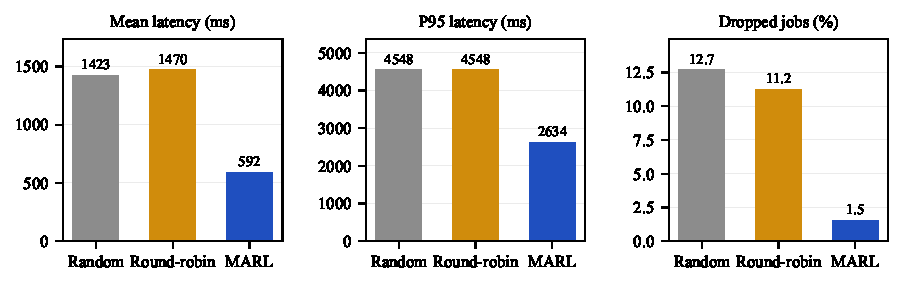
\includegraphics[width=0.92\textwidth]{figures/results.pdf}
\caption{Mean latency, P95 latency and rejected-job rate per policy over the measurement window.}
\label{fig:results}
\end{figure*}

\subsection{Learning dynamics}
Fig.~\ref{fig:curve} plots 5-second averages over each full run. Starting from a uniformly random policy, the MARL agents' latency fell below 400~ms within about 30~s, while $\varepsilon$ was still decaying. $\varepsilon$ reached its floor of 0.02 after 43~s, close to the expected $\ln 0.02 / \ln 0.995 \approx 780$ decisions at 17 decisions/s (46~s). After their first 10~s, the baselines stayed between roughly 1.0 and 1.7~s.

Even after convergence, MARL shows occasional latency spikes, for example near 87~s and 117~s, the second with a brief 10\% rejection rate. The agents act on load snapshots up to 100~ms old and do not see each other's in-flight decisions. Several agents can therefore move to the same VM at once, which is the herd effect of stale load information~\cite{mitzenmacher2000old} seen from a learning perspective. In a separate live run we observed a 4-slot VM briefly holding 17 jobs for this reason. The small rise in $\varepsilon$ near 52~s comes from a load poll that failed under load, which an agent treated as a health change.

\begin{figure}[t]
\centering
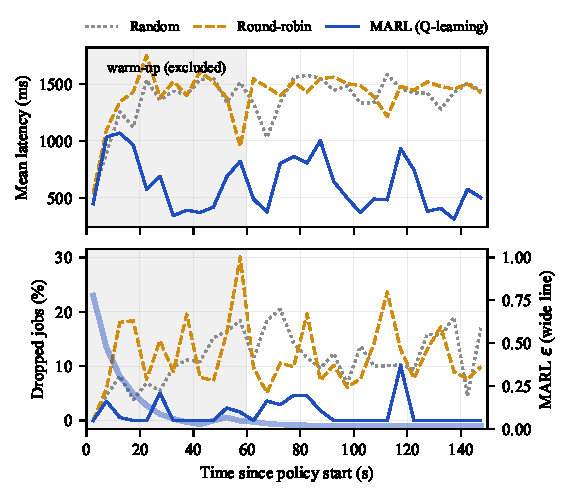
\includegraphics[width=\columnwidth]{figures/learning_curve.pdf}
\caption{Mean latency (top) and rejected-job rate (bottom) in 5-s bins for each policy, with the MARL agents' average exploration rate $\varepsilon$ (bottom, wide line). The shaded warm-up period is excluded from Table~\ref{tab:results}.}
\label{fig:curve}
\end{figure}

\subsection{What the agents learned}
Table~\ref{tab:share} shows each region's routing split in the measurement window. Round-robin sent $20.0\pm0.2\%$ of every region's jobs to every VM. The MARL agents moved traffic off the two small VMs (13.7\% and 12.8\% on average) and toward the larger ones. They also learned proximity: Frankfurt's most-used VM is its nearest one, vm-m (30~ms), Singapore's is vm-l (30~ms), and Mumbai's is vm-xl (30~ms). Mumbai's nearest VM, vm-s1 (20~ms), receives only 14.0\% of its jobs because it has only two slots. The agents therefore balance network delay against queueing delay without being told either.

The learned allocation is not capacity-proportional. A split proportional to capacity would be 35/25/20/10/10\%. The implied utilizations in Table~\ref{tab:share} show that vm-xl stays at 0.51 while the small VMs run at 0.87--0.93, close to saturation. The coarse three-level state cannot tell a nearly full small VM from a moderately loaded large one, and the agents are not rewarded for spare capacity, so they stop shifting load once latency is acceptable. A finer state, or a shared reward that includes pool-wide latency, could close this gap.

\begin{table}[t]
\caption{Learned routing split (\% of each region's jobs, 60--150 s)}
\label{tab:share}
\centering
\begin{tabular}{@{}lccccc@{}}
\toprule
Region & vm-xl & vm-l & vm-m & vm-s1 & vm-s2 \\
\midrule
Mumbai    & \textbf{31.3} & 26.0 & 19.4 & 14.0 & 9.4 \\
Singapore & 26.9 & \textbf{30.2} & 16.7 & 13.2 & 13.0 \\
Frankfurt & 22.0 & 23.4 & \textbf{26.5} & 14.2 & 13.8 \\
Virginia  & 24.5 & 22.4 & \textbf{24.9} & 13.3 & 14.9 \\
\midrule
Mean (MARL)           & 26.2 & 25.5 & 21.9 & 13.7 & 12.8 \\
Capacity share        & 35.0 & 25.0 & 20.0 & 10.0 & 10.0 \\
\midrule
Utilization, MARL     & 0.51 & 0.69 & 0.74 & 0.93 & 0.87 \\
Utilization, RR       & 0.39 & 0.54 & 0.68 & 1.36 & 1.36 \\
\bottomrule
\end{tabular}
\\[2pt]{\footnotesize Utilization $=$ offered rate (68 jobs/s $\times$ share) / max rate.}
\end{table}

\subsection{Behaviour under VM failure}
In an exploratory run (not part of the controlled comparison), we took vm-l down after the agents had converged. The health change raised $\varepsilon$ to about 0.2, and within tens of seconds the agents' share of traffic sent to vm-l fell from 20--30\% to 6--8\%. Mean latency nevertheless rose to roughly 0.9--1.6~s, because losing 25 jobs/s of capacity left the remaining pool at about 91\% utilization, a regime in which every policy suffers. We did not test failures of the small VMs in a controlled way.

\subsection{Limitations}
Several factors limit the generality of these results. (i) Each policy was measured in a single run, so no confidence intervals are reported. (ii) Network delay was emulated, and all services shared one host, so CPU contention and timer resolution affect absolute latencies. (iii) The baselines ignore capacity and health. Weighted round-robin, least-connections and power-of-two-choices~\cite{mitzenmacher2001} are stronger comparisons and would narrow the gap. (iv) MARL was measured after a 60~s warm-up; during roughly the first 20~s its performance resembles that of random routing. (v) The tabular state does not scale to large pools.

\section{Conclusion and Future Work}
CloudMARL shows that very simple independent Q-learning agents, one per regional load balancer and with no communication, can learn within a minute to route around small VMs and toward nearby capacity. In our testbed this cut mean latency by 58.4\% and rejected jobs from about 12\% to 1.5\% compared with capacity-blind baselines. The study also exposes the typical weaknesses of independent learners: herding on shared snapshots and convergence to an allocation that is good but not capacity-proportional.

Future work includes comparison with weighted and queue-aware baselines over repeated runs, a cooperative reward based on pool-wide latency, function approximation (DQN~\cite{mnih2015dqn}) or centralized-training methods such as MADDPG~\cite{lowe2017maddpg} for larger pools, and deployment on genuinely geo-distributed cloud regions instead of emulated delay.

\section*{Code Availability}
The source code, deployment scripts, Grafana dashboard and experiment scripts are available at \url{https://github.com/anuranbaruah/cloudmarl-load-balancer}.

\begin{thebibliography}{00}
\bibitem{mitzenmacher2001} M. Mitzenmacher, ``The power of two choices in randomized load balancing,'' \textit{IEEE Trans. Parallel Distrib. Syst.}, vol.~12, no.~10, pp.~1094--1104, Oct. 2001.
\bibitem{mitzenmacher2000old} M. Mitzenmacher, ``How useful is old information?'' \textit{IEEE Trans. Parallel Distrib. Syst.}, vol.~11, no.~1, pp.~6--20, Jan. 2000.
\bibitem{lu2011jiq} Y. Lu, Q. Xie, G. Kliot, A. Geller, J. R. Larus, and A. Greenberg, ``Join-Idle-Queue: A novel load balancing algorithm for dynamically scalable web services,'' \textit{Performance Evaluation}, vol.~68, no.~11, pp.~1056--1071, 2011.
\bibitem{sutton2018} R. S. Sutton and A. G. Barto, \textit{Reinforcement Learning: An Introduction}, 2nd~ed. Cambridge, MA, USA: MIT Press, 2018.
\bibitem{mao2016deeprm} H. Mao, M. Alizadeh, I. Menache, and S. Kandula, ``Resource management with deep reinforcement learning,'' in \textit{Proc. 15th ACM Workshop on Hot Topics in Networks (HotNets)}, 2016, pp.~50--56.
\bibitem{busoniu2008} L. Bu\c{s}oniu, R. Babu\v{s}ka, and B. De Schutter, ``A comprehensive survey of multiagent reinforcement learning,'' \textit{IEEE Trans. Syst., Man, Cybern. C}, vol.~38, no.~2, pp.~156--172, Mar. 2008.
\bibitem{hernandezleal2017} P. Hernandez-Leal, M. Kaisers, T. Baarslag, and E. Munoz de Cote, ``A survey of learning in multiagent environments: Dealing with non-stationarity,'' arXiv:1707.09183, 2017.
\bibitem{tan1993} M. Tan, ``Multi-agent reinforcement learning: Independent vs. cooperative agents,'' in \textit{Proc. 10th Int. Conf. Machine Learning (ICML)}, 1993, pp.~330--337.
\bibitem{claus1998} C. Claus and C. Boutilier, ``The dynamics of reinforcement learning in cooperative multiagent systems,'' in \textit{Proc. 15th National Conf. Artificial Intelligence (AAAI)}, 1998, pp.~746--752.
\bibitem{eisenbud2016maglev} D. E. Eisenbud \textit{et al.}, ``Maglev: A fast and reliable software network load balancer,'' in \textit{Proc. 13th USENIX Symp. Networked Systems Design and Implementation (NSDI)}, 2016, pp.~523--535.
\bibitem{watkins1992} C. J. C. H. Watkins and P. Dayan, ``Q-learning,'' \textit{Machine Learning}, vol.~8, no.~3--4, pp.~279--292, 1992.
\bibitem{mnih2015dqn} V. Mnih \textit{et al.}, ``Human-level control through deep reinforcement learning,'' \textit{Nature}, vol.~518, no.~7540, pp.~529--533, 2015.
\bibitem{lowe2017maddpg} R. Lowe, Y. Wu, A. Tamar, J. Harb, P. Abbeel, and I. Mordatch, ``Multi-agent actor-critic for mixed cooperative-competitive environments,'' in \textit{Proc. Advances in Neural Information Processing Systems (NeurIPS)}, 2017, pp.~6379--6390.
\end{thebibliography}

\end{document}
